\chapter{Química bioinorgânica}\label{ch:b3:bioinorganic}

Nosso sangue é vermelho por causa do ferro; o sangue de um límulo é incolor em
suas veias e fica azul ao ar, porque transporta o oxigênio sobre o cobre. A vida usa
um punhado de íons metálicos para as tarefas que nenhum grupo orgânico consegue fazer: ligar o oxigênio
de modo reversível, deslocar elétrons um a um, quebrar a água, reduzir o nitrogênio,
tornar uma molécula de água ácida o bastante para atacar o dióxido de carbono. Este capítulo
lê essas tarefas com as ferramentas da química de coordenação: \omterm{def:b3:bioinorganic:hsab}{ácidos duros} e
moles, campos ligantes e estados de spin, equilíbrios e leis de velocidade, e termina
com os metais usados como fármacos.

\begin{recall}
O volume do 2.º ano tratou dos $\alpha$-aminoácidos, das cadeias laterais e dos peptídeos, das nucleobases
e dos nucleotídeos, dos complexos de coordenação, dos campos ligantes, do spin alto e baixo, e dos
nucleófilos e eletrófilos duros e moles; o volume do 1.º ano, das constantes de
complexação e da escala de pL. O \cref{ch:b3:complex-spectra-magnetism} e o
\cref{ch:b3:complex-mechanisms} deram os espectros, a teoria de Marcus e a aquação da
cisplatina, o \cref{ch:b3:complex-kinetics}, a cinética de Michaelis--Menten, e o
\cref{ch:b3:advanced-nmr}, o tempo de relaxação $T_1$.
\end{recall}

\begin{omfigure}
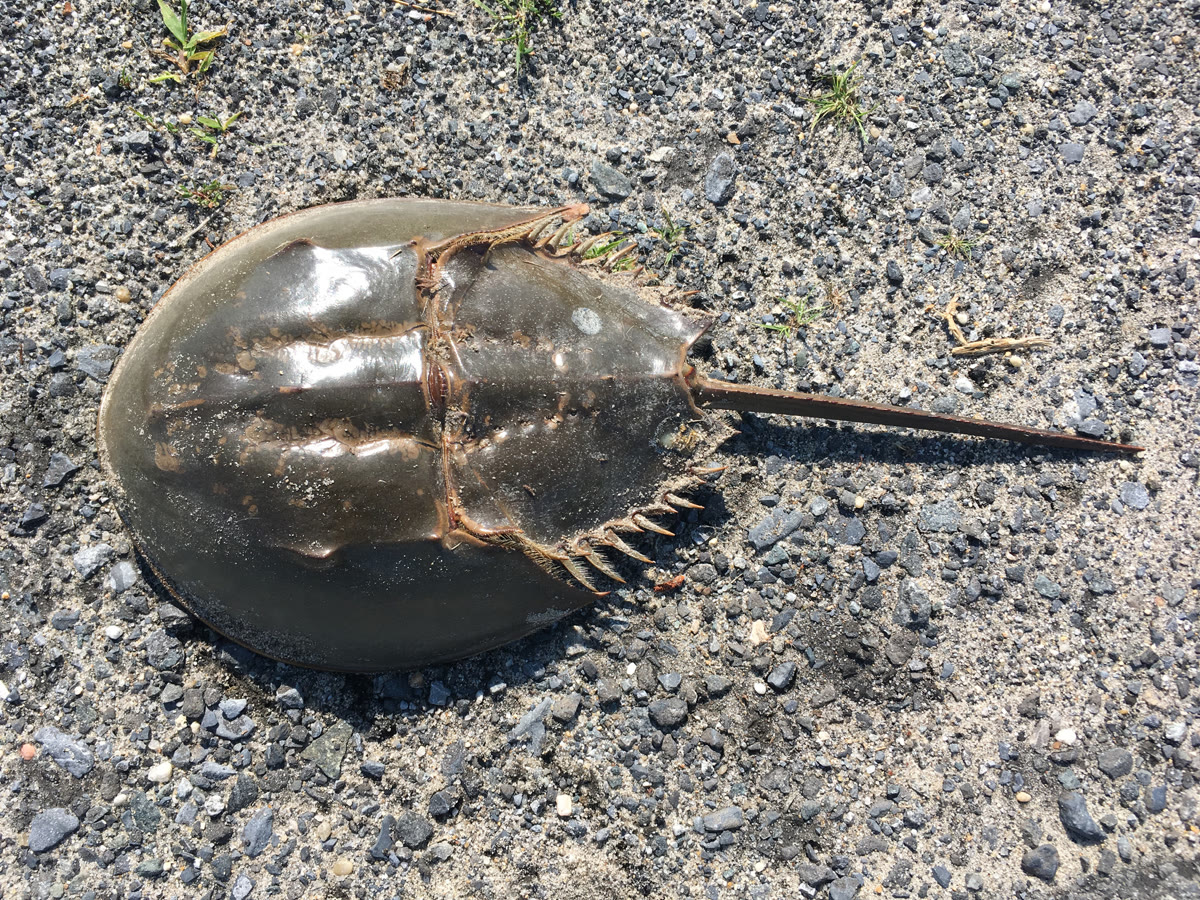
\includegraphics[width=0.5\linewidth]{images/book4/horseshoe-crab.jpg}

{\small Um límulo do Atlântico. Seu sangue transporta o oxigênio sobre a hemocianina, uma
proteína de cobre, e é azul quando oxigenado. Fotografia: Kaldari, CC0.}
\end{omfigure}

\section{Os metais na biologia}

\begin{definition}[Metaloproteínas]\label{def:b3:bioinorganic:metalloprotein}
Uma \emph{metaloproteína}\index{metaloproteina@metaloproteína} é uma proteína que contém
íons metálicos ligados; uma \emph{metaloenzima}\index{metaloenzima} é uma metaloproteína que
catalisa uma reação. Um \emph{cofator}\index{cofator} é uma espécie não proteica,
um íon metálico ou uma molécula pequena, ligada a uma proteína e necessária à sua
atividade.
\end{definition}

Os metais que importam em quantidade são o sódio, o potássio, o magnésio e o
cálcio, que sobretudo transportam carga e sustentam estruturas; os metais de transição
ferro, zinco, cobre, manganês, cobalto, molibdênio e níquel ocorrem em traços,
mas comandam boa parte da química. Uma proteína escolhe seu metal pelos átomos
doadores que oferece e por sua geometria.

\begin{definition}[Ácidos duros e moles]\label{def:b3:bioinorganic:hsab}
Um \emph{ácido duro}\index{acido duro@ácido duro} é um ácido de Lewis pequeno, muito carregado, pouco
polarizável ($\ce{H+}$, $\ce{Mg^2+}$, $\ce{Ca^2+}$, $\ce{Fe^3+}$); um \emph{ácido
mole}\index{acido mole@ácido mole} é um ácido grande, polarizável e de carga baixa ($\ce{Cu+}$, $\ce{Ag+}$,
$\ce{Hg^2+}$, $\ce{Cd^2+}$). O \emph{princípio dos ácidos e bases duros e moles}\index{principio dos acidos e bases duros e moles@princípio dos ácidos e bases duros e moles}
afirma que os ácidos duros se ligam preferencialmente às bases duras
(doadores de oxigênio, fluoreto) e os ácidos moles às bases moles (doadores de enxofre, iodeto).
\end{definition}

Nas proteínas, os carboxilatos e os fenolatos são duros, o tiolato da cisteína e
o tioéter da metionina, moles, e o imidazol da histidina, intermediário. O ferro(III)
fica entre doadores de oxigênio, o cobre(I) entre doadores de enxofre, o zinco, um ácido
intermediário, com histidina e cisteína; o mercúrio e o cádmio são tóxicos em parte
porque capturam as cisteínas das \omterm{def:b3:complex-kinetics:enzyme}{enzimas}.

\begin{definition}[Série de Irving--Williams]\label{def:b3:bioinorganic:irving-williams}
A \emph{série de Irving--Williams}\index{serie de Irving--Williams@série de Irving--Williams} é a ordem
de estabilidade dos complexos de spin alto dos íons divalentes da primeira
série de transição com um dado ligante:
$\ce{Mn^2+} < \ce{Fe^2+} < \ce{Co^2+} < \ce{Ni^2+} < \ce{Cu^2+} > \ce{Zn^2+}$.
\end{definition}

\begin{proposition}[Ordem de Irving--Williams]\label{prop:b3:bioinorganic:irving-williams}
A série vale para quase todos os ligantes (uma observação experimental); ela
acompanha a diminuição do raio iônico do manganês ao cobre, a energia de estabilização
do campo ligante, nula para $d^5$, máxima para $d^8$, e a distorção de Jahn--Teller
do cobre(II), que encurta quatro de suas ligações.
\end{proposition}

\begin{proof}[Argumento]
O raio diminui ao longo da série à medida que a carga nuclear cresce, o que reforça
a atração eletrostática de todo ligante. A estabilização do campo ligante dos
íons octaédricos de spin alto (\cref{ch:b3:complex-spectra-magnetism}) é $0$, $4$,
$8$, $12$ e $6\,\mathrm{Dq}$ de $d^5$ a $d^9$, e $0$ para $d^{10}$: ela reforça a tendência até o níquel e
cai para o zinco; o cobre(II) recupera mais do que sua estabilização sugere por
sua distorção tetragonal, que dá quatro ligações curtas e fortes.
\end{proof}

Uma consequência que as células precisam gerenciar: o cobre e o zinco desbancariam os
outros íons na maioria dos sítios, de modo que suas concentrações livres são mantidas extremamente baixas
por proteínas transportadoras dedicadas.

\section{O transporte de oxigênio}

\begin{definition}[Porfirinas e heme]\label{def:b3:bioinorganic:haem}
Uma \emph{porfirina}\index{porfirina} é um macrociclo aromático grande e plano de quatro
anéis pirrol unidos por pontes metino, cujos quatro nitrogênios ligam um íon metálico
em seu centro. O \emph{heme}\index{heme} é o complexo de ferro da protoporfirina~IX,
o \omterm{def:b3:bioinorganic:metalloprotein}{cofator} da hemoglobina, da mioglobina e dos citocromos.
\end{definition}

Na mioglobina e na hemoglobina, o ferro do \omterm{def:b3:bioinorganic:haem}{heme} tem um quinto ligante abaixo do
anel, o nitrogênio da histidina proximal, e um sexto sítio livre para o $\ce{O2}$.
O ferro(II) desóxi é de spin alto: um elétron no orbital $d_{x^2-y^2}$, que aponta para os quatro
nitrogênios, o torna grande demais para o buraco do anel, e ele fica fora do
plano, do lado da histidina. Ao ligar o $\ce{O2}$, ele passa a spin baixo, menor, e
entra no plano, puxando consigo a histidina e a hélice da proteína.

\begin{omfigure}
% ledger: pdb:Hb.deoxy.FeN4, pdb:Hb.oxy.FeN4
\begin{tikzpicture}[font=\small, scale=0.9]
  \foreach \x/\lab/\dz/\oxy in {0/desóxi (spin alto)/-0.34/0, 6.4/óxi (spin baixo)/-0.04/1} {
    \begin{scope}[xshift=\x cm]
      \draw[omDef, line width=2.6pt] (-2.2,0) -- (2.2,0);
      \node[font=\scriptsize, anchor=west, omDef] at (2.3,0) {porfirina};
      \fill[omThm] (0,\dz*1.5) circle (0.22);
      \node[font=\scriptsize, anchor=north west] at (0.2,\dz*1.5-0.12) {Fe};
      \draw[black!70, line width=1pt] (0,\dz*1.5-0.22) -- (0,-1.55);
      \node[draw=black!70, regular polygon, regular polygon sides=5, minimum size=7mm, inner sep=0pt] at (0,-1.95) {};
      \node[font=\scriptsize, anchor=west] at (0.45,-1.95) {His proximal};
      \node[font=\small\bfseries] at (0,1.9) {\lab};
      \ifnum\oxy=1
        \draw[black!70, line width=1pt] (0,0.2) -- (0,0.85) -- (0.55,1.25);
        \fill[red!75] (0,0.85) circle (0.13) (0.55,1.25) circle (0.13);
        \node[font=\scriptsize, anchor=west] at (0.75,1.2) {$\ce{O2}$, angular};
      \fi
    \end{scope}
  }
  \draw[<->, black!60] (-1.0,0) -- (-1.0,-0.51) node[midway, left, font=\scriptsize] {\qty{0.34}{\angstrom}};
\end{tikzpicture}

{\small O ferro do \omterm{def:b3:bioinorganic:haem}{heme} visto de perfil, com seu deslocamento em relação ao anel desenhado em
escala (1~\AA{} para 1.35~cm; as demais distâncias são esquemáticas). Na desoxi-hemoglobina, o ferro(II) de spin alto fica
\qty{0.34}{\angstrom} abaixo do plano médio dos quatro nitrogênios pirrólicos, do lado da
histidina proximal; na oxi-hemoglobina, ele fica a menos de \qty{0.05}{\angstrom} do plano, com o $\ce{O2}$
ligado pela extremidade e angular (distâncias calculadas a partir de estruturas cristalinas).}
\end{omfigure}

O dioxigênio ligado é mais bem descrito como superóxido sobre ferro(III), $\ce{Fe^{III}-O2^-}$, do que como
$\ce{O2}$ neutro sobre ferro(II): o complexo é diamagnético porque os elétrons
desemparelhados dos dois centros se acoplam. A proteína impede a oxidação
irreversível a ferro(III) e água, que um \omterm{def:b3:bioinorganic:haem}{heme} isolado em água sofre
imediatamente.

\begin{definition}[Ligação cooperativa]\label{def:b3:bioinorganic:cooperativity}
A ligação a uma proteína com vários sítios é uma \emph{ligação cooperativa}\index{ligacao cooperativa@ligação cooperativa}
quando a ligação de um ligante aumenta a afinidade dos sítios
restantes. O \emph{coeficiente de Hill}\index{coeficiente de Hill} $n$ é a inclinação do
gráfico de Hill, $\log\frac{\theta}{1 - \theta}$ em função de $\log p$, na meia-saturação ($\theta$ é a fração de sítios
ocupados).
\end{definition}

\begin{proposition}[Um único sítio]\label{prop:b3:bioinorganic:hyperbola}
Para uma proteína com um sítio, $\mathrm{P + O_2 \rightleftharpoons PO_2}$, a fração ocupada é $\theta = p/(p_{50} + p)$, onde $p_{50}$ é
a constante de dissociação expressa como pressão.
\end{proposition}

\begin{proof}
$K_d = [\mathrm P]p/[\mathrm{PO_2}] = p_{50}$, logo $[\mathrm{PO_2}] = [\mathrm P]p/p_{50}$, e $\theta = [\mathrm{PO_2}]/([\mathrm P] + [\mathrm{PO_2}]) = (p/p_{50})/(1 + p/p_{50})$.
\end{proof}

\begin{theorem}[Equação de Hill]\label{thm:b3:bioinorganic:hill}
Para uma proteína com $n$ sítios que estão ou todos vazios ou todos ocupados,
$\mathrm{P + n\,O_2 \rightleftharpoons P(O_2)_n}$,
\[
  \theta = \frac{p^n}{p_{50}^n + p^n}, \qquad \log\frac{\theta}{1 - \theta} = n\log p - n\log p_{50}.
\]
\end{theorem}

\begin{proof}
$K_d = [\mathrm P]p^n/[\mathrm{P(O_2)_n}]$; escreva $K_d = p_{50}^n$. A fração de sítios ocupados é a de moléculas
na forma ocupada, $\theta = [\mathrm{P(O_2)_n}]/([\mathrm P] + [\mathrm{P(O_2)_n}]) = (p/p_{50})^n/(1 + (p/p_{50})^n)$. Então $\theta/(1 - \theta) = (p/p_{50})^n$, e tomando os
logaritmos obtém-se a reta de inclinação $n$.
\end{proof}

A hemoglobina, com quatro sítios, não é totalmente cooperativa: seu \omterm{def:b3:bioinorganic:cooperativity}{coeficiente de Hill} fica
bem abaixo de 4, em torno de 3, e seu gráfico de Hill tem inclinação 1 nas duas extremidades, onde
ela se comporta como uma proteína desóxi ou óxi de sítios independentes. A
cooperatividade vem de uma mudança de estrutura quaternária: o movimento do
ferro para o plano do primeiro \omterm{def:b3:bioinorganic:haem}{heme} a ligar o $\ce{O2}$ é transmitido às outras subunidades.

\begin{omfigure}
\begin{tikzpicture}
\begin{axis}[name=a, width=0.48\linewidth, height=5.6cm, xmin=0, xmax=14, ymin=0, ymax=1.02,
  axis lines=left, xlabel={$p(\ce{O2})$ / \unit{kPa}}, ylabel={saturação $\theta$},
  tick label style={font=\scriptsize}, label style={font=\small}]
\addplot[omMeth, thick] table[x=p, y=Mb] {figdata/out/bachelor-3-oxygen-binding.dat};
\addplot[omThm, thick] table[x=p, y=Hb] {figdata/out/bachelor-3-oxygen-binding.dat};
\addplot[omThm, thick, dashed] table[x=p, y=Hbacid] {figdata/out/bachelor-3-oxygen-binding.dat};
\draw[black!35] (axis cs:5,0) -- (axis cs:5,1.0) (axis cs:13,0) -- (axis cs:13,1.0);
\node[font=\scriptsize, anchor=south] at (axis cs:5,0.02) {tecidos};
\node[font=\scriptsize, anchor=south east] at (axis cs:13,0.02) {pulmões};
\node[font=\scriptsize, omMeth] at (axis cs:1.9,0.96) {Mb};
\node[font=\scriptsize, omThm] at (axis cs:7.5,0.6) {Hb};
\end{axis}
\begin{axis}[at={(a.east)}, anchor=west, xshift=1.4cm, width=0.48\linewidth, height=5.6cm,
  xmin=-1.5, xmax=1.5, ymin=-3, ymax=3, axis lines=left,
  xlabel={$\log_{10}(p/\unit{kPa})$}, ylabel={$\log_{10}\bigl(\theta/(1-\theta)\bigr)$},
  tick label style={font=\scriptsize}, label style={font=\small}]
\draw[black!30] (axis cs:-1.5,0) -- (axis cs:1.5,0);
\addplot[omMeth, thick] table[x=lgp, y=Mb] {figdata/out/bachelor-3-oxygen-binding-b.dat};
\addplot[omThm, thick, restrict y to domain=-3:3] table[x=lgp, y=Hb] {figdata/out/bachelor-3-oxygen-binding-b.dat};
\node[font=\scriptsize, omMeth, anchor=west] at (axis cs:-1.1,1.4) {inclinação 1};
\node[font=\scriptsize, omThm, anchor=west] at (axis cs:0.75,-1.5) {\shortstack[l]{inclinação\\ 2.7}};
\end{axis}
\end{tikzpicture}

{\small À esquerda: saturação em oxigênio da mioglobina (verde) e da hemoglobina (vermelho;
tracejado: a pH mais baixo) em função da pressão de oxigênio, com os valores do modelo
$p_{50} = \qty{0.37}{kPa}$ (Mb) e \qty{3.5}{kPa} (Hb), $n = 2.7$. Entre os pulmões e os tecidos, a hemoglobina
cede um quarto de seu oxigênio, a mioglobina quase nada. À direita: os
gráficos de Hill correspondentes, retas neste modelo (o gráfico da hemoglobina real
se curva para inclinação 1 nas duas extremidades).}
\end{omfigure}

\begin{method}[Ler um gráfico de Hill]\label{met:b3:bioinorganic:hill-plot}
\begin{enumerate}
  \item A partir de cada saturação medida, calcule $\log(\theta/(1 - \theta))$; trace-o em função de $\log p$.
  \item A pressão em que o gráfico cruza o zero é $p_{50}$.
  \item A inclinação nesse ponto é o \omterm{def:b3:bioinorganic:cooperativity}{coeficiente de Hill}: $n = 1$ significa sítios
        independentes, $n > 1$, \omterm{def:b3:bioinorganic:cooperativity}{ligação cooperativa}.
  \item Com apenas dois pontos, $n = \Delta\log(\theta/(1 - \theta))/\Delta\log p$.
\end{enumerate}
\end{method}

A hemoglobina também liga prótons e dióxido de carbono em sítios afastados do \omterm{def:b3:bioinorganic:haem}{heme},
o que desloca sua curva para a direita onde eles são abundantes, nos tecidos em atividade:
o efeito Bohr libera mais oxigênio exatamente onde ele é necessário.

\begin{proposition}[Competição com o monóxido de carbono]\label{prop:b3:bioinorganic:haldane}
Se o monóxido de carbono e o dioxigênio competem pelos mesmos sítios, com
$\mathrm{HbO_2 + CO \rightleftharpoons HbCO + O_2}$ de constante de equilíbrio $M$, então
$[\mathrm{HbCO}]/[\mathrm{HbO_2}] = M\,p(\ce{CO})/p(\ce{O2})$.
\end{proposition}

\begin{proof}
No equilíbrio, $M = [\mathrm{HbCO}]\,p(\ce{O2})/([\mathrm{HbO_2}]\,p(\ce{CO}))$; rearranjando, obtém-se o resultado.
\end{proof}

$M$ é da ordem das centenas para a hemoglobina humana, de modo que algumas centenas de partes por
milhão de monóxido de carbono ocupam uma grande fração dos sítios; pior, os
sítios que ficam livres retêm seu oxigênio mais firmemente, pois a cooperatividade
age sobre eles. O \omterm{def:b3:bioinorganic:haem}{heme} livre liga o monóxido de carbono muito mais fortemente ainda: na
proteína, uma histidina distal acima do ferro dificulta a geometria linear Fe--C--O
que o monóxido de carbono prefere, ao passo que faz ligação de hidrogênio com o $\ce{O2}$ angular.
Outros animais usam outros metais: as hemocianinas dos moluscos e dos artrópodes
ligam o $\ce{O2}$ entre dois íons cobre na forma de peróxido, as hemeritrinas de alguns
vermes marinhos, sobre um par de íons ferro.

\begin{inthelab}[Uma curva de ligação do oxigênio]
Uma solução de hemoglobina em tampão é colocada em uma cubeta estanque a gases provida
de um balão lateral. Ela é primeiro livrada do oxigênio por purga com nitrogênio; depois,
volumes conhecidos de ar são injetados e a solução é equilibrada por leve
inclinação. Após cada adição, registra-se o espectro visível: as bandas da
forma desóxi (uma banda perto de \qty{555}{nm}) dão lugar às duas bandas da forma óxi,
e a saturação é lida pela absorbância em um comprimento de onda, entre seus limites
desóxi e óxi.
\end{inthelab}

\section{Metaloenzimas}

A anidrase carbônica acelera $\ce{CO2 + H2O <=> HCO3- + H+}$, que em água pura leva
segundos, o suficiente para importar na curta passagem da hemácia por um capilar
pulmonar. Seu íon zinco é mantido por três histidinas e uma molécula de água. Cátion
pequeno e de carga alta, ele abaixa o $\mathrm pK_a$ dessa água de cerca de 14 para
cerca de 7: em pH fisiológico, boa parte da \omterm{def:b3:complex-kinetics:enzyme}{enzima} carrega um hidróxido ligado ao zinco,
um nucleófilo forte, mantido bem ao lado de uma cavidade que liga o $\ce{CO2}$.

\begin{omfigure}
\begin{tikzpicture}[font=\small, >=Stealth]
  \node (a) at (90:2.0) {$\mathrm{(His)_3Zn{-}OH_2}$};
  \node (b) at (0:2.9) {$\mathrm{(His)_3Zn{-}OH^-}$};
  \node (c) at (-90:2.0) {$\mathrm{(His)_3Zn{-}OCO_2H^-}$};
  \draw[->, thick] (a) to[bend left=25] node[midway, above right, font=\scriptsize] {$-\,\ce{H+}$ (para uma histidina transportadora)} (b);
  \draw[->, thick] (b) to[bend left=25] node[midway, below right, font=\scriptsize, align=left] {$+\,\ce{CO2}$:\\ ataque nucleofílico} (c);
  \draw[->, thick] (c) to[bend left=35] node[midway, left, font=\scriptsize, align=right] {$+\,\ce{H2O}$\\ $-\,\ce{HCO3-}$} (a);
\end{tikzpicture}

{\small O ciclo catalítico da anidrase carbônica. A água ligada ao zinco perde um
próton; o hidróxido ligado ao zinco ataca o dióxido de carbono; a água desloca o
hidrogenocarbonato. A transferência de próton para o solvente é a etapa mais lenta.}
\end{omfigure}

\begin{proposition}[Uma enzima rápida]\label{prop:b3:bioinorganic:carbonic-anhydrase}
A \omterm{def:b3:complex-kinetics:michaelis}{constante de especificidade} $k_{\mathrm{cat}}/K_M$ da anidrase carbônica se aproxima da constante
de velocidade de encontro do $\ce{CO2}$ com a \omterm{def:b3:complex-kinetics:enzyme}{enzima}: quase todo encontro leva à
reação.
\end{proposition}

\begin{proof}[Argumento]
$k_{\mathrm{cat}}/K_M$ é a constante de velocidade de segunda ordem da \omterm{def:b3:complex-kinetics:enzyme}{enzima} com o substrato a baixa
concentração de substrato (\cref{ch:b3:complex-kinetics}); ela não pode exceder a
constante de velocidade, \omterm{def:b3:rate-theories:diffusion}{controlada por difusão}, de seu encontro
(\cref{ch:b3:rate-theories}). Os valores medidos para a anidrase carbônica estão
entre os mais altos conhecidos para qualquer \omterm{def:b3:complex-kinetics:enzyme}{enzima} e se aproximam desse limite: a química
dentro do \omterm{def:b3:complex-kinetics:enzyme}{sítio ativo} deixa então de ser o que limita a velocidade.
\end{proof}

As \omterm{def:b3:complex-kinetics:enzyme}{enzimas} do citocromo P450, no fígado e em muitas outras células, hidroxilam ligações C--H
de fármacos e hormônios. Seu ferro hemínico é mantido por um tiolato de cisteína; com
$\ce{O2}$ e dois elétrons, ele forma um complexo ferro(IV)-oxo com um radical na
\omterm{def:b3:bioinorganic:haem}{porfirina}, chamado composto I, que abstrai um átomo de hidrogênio do
substrato e devolve o grupo hidroxila ao radical carbonado. A nitrogenase
reduz o $\ce{N2}$ a amônia à temperatura ambiente em um agregado de sete átomos de ferro,
um de molibdênio e nove sulfetos em torno de um átomo de carbono central, o \omterm{def:b3:bioinorganic:metalloprotein}{cofator}
FeMo, ao custo de muitas moléculas de ATP. A vitamina $\mathrm{B_{12}}$ contém uma
ligação cobalto--carbono, uma das pouquíssimas ligações metal--carbono da biologia, cuja
homólise inicia rearranjos radicalares.

\section{Transferência de elétrons e energia}

As proteínas que apenas transportam elétrons têm centros metálicos com pequenas
\omterm{def:b3:complex-mechanisms:reorganisation}{energias de reorganização} (\cref{ch:b3:complex-mechanisms}): os dois estados de
oxidação têm quase a mesma geometria, de modo que a barreira de Marcus é baixa.

\begin{definition}[Centros ferro--enxofre]\label{def:b3:bioinorganic:fes}
Um \emph{centro ferro--enxofre}\index{centro ferro--enxofre} é um grupo de íons
ferro unidos em ponte por íons sulfeto e ligados à proteína por tiolatos de cisteína:
$\ce{[2Fe-2S]}$, $\ce{[3Fe-4S]}$ e o $\ce{[4Fe-4S]}$, de tipo cubano.
\end{definition}

\begin{definition}[Proteínas de cobre azul]\label{def:b3:bioinorganic:blue-copper}
Uma \emph{proteína de cobre azul}\index{proteina de cobre azul@proteína de cobre azul} contém um íon
cobre ligado a duas histidinas, a uma cisteína e a uma metionina fracamente ligada em um
sítio tetraédrico distorcido; sua intensa cor azul vem de uma
banda de transferência de carga cisteína--cobre(II).
\end{definition}

\begin{definition}[Estado entático]\label{def:b3:bioinorganic:entatic}
O \emph{estado entático}\index{estado entatico@estado entático} é um sítio metálico mantido pela
proteína em uma geometria tensionada, intermediária entre as geometrias preferidas por seus dois
estados de oxidação, o que abaixa a \omterm{def:b3:complex-mechanisms:reorganisation}{energia de reorganização} de suas reações.
\end{definition}

O cobre(II) sozinho prefere um quadrado plano, o cobre(I) um tetraedro: no sítio de cobre
azul, nenhum dos dois é satisfeito, e a transferência de elétrons é rápida.

\begin{definition}[Complexo de evolução de oxigênio]\label{def:b3:bioinorganic:oec}
O \emph{complexo de evolução de oxigênio}\index{complexo de evolucao de oxigenio@complexo de evolução de oxigênio} do
fotossistema~II é o agregado $\mathrm{Mn_4CaO_5}$ que oxida a água a dioxigênio na
fotossíntese.
\end{definition}

\begin{proposition}[Quatro fótons por oxigênio]\label{prop:b3:bioinorganic:kok}
Oxidar duas moléculas de água a um $\ce{O2}$ exige quatro fótons absorvidos pelo
fotossistema~II, passando o agregado por cinco estados, de $\mathrm S_0$ a $\mathrm S_4$.
\end{proposition}

\begin{proof}
$\ce{2H2O -> O2 + 4H+ + 4e-}$: quatro elétrons precisam ser retirados. Cada fóton absorvido pelo
centro de reação afasta dele um elétron, e o agregado repõe o centro
oxidado um elétron por vez: quatro fótons, quatro etapas, armazenando
equivalentes oxidantes nos estados $\mathrm S_1$ a $\mathrm S_4$; $\mathrm S_4$ libera o $\ce{O2}$ e volta a $\mathrm S_0$.
\end{proof}

\begin{omfigure}
\begin{tikzpicture}[font=\small, >=Stealth]
  \foreach \i/\ang in {0/90, 1/18, 2/-54, 3/-126, 4/162} {
    \node[draw, circle, minimum size=9mm, fill=omDef!10] (s\i) at (\ang:2.0) {$\mathrm S_{\i}$};
  }
  \foreach \i/\j in {0/1, 1/2, 2/3, 3/4} {
    \draw[->, thick] (s\i) to[bend left=18] node[midway, sloped, above, font=\scriptsize] {$h\nu$, $-\mathrm e^-$} (s\j);
  }
  \draw[->, thick, omThm] (s4) to[bend left=18] node[midway, sloped, above, font=\scriptsize] {$-\ce{O2}$, $+\,\ce{2H2O}$} (s0);
\end{tikzpicture}

{\small O ciclo de Kok do \omterm{def:b3:bioinorganic:oec}{complexo de evolução de oxigênio}. Cada fóton absorvido pelo
fotossistema~II retira um elétron do agregado de manganês (os prótons
saem no caminho); a quarta oxidação dá $\mathrm S_4$, que libera o dioxigênio e
volta a ligar duas moléculas de água.}
\end{omfigure}

Na outra ponta da cadeia energética, a citocromo $c$ oxidase das
mitocôndrias reduz o $\ce{O2}$ a água com quatro elétrons e quatro prótons em um
ferro hemínico e um íon cobre frente a frente, sem liberar o superóxido ou o peróxido,
parcialmente reduzidos e nocivos.

\section{Os metais na medicina}

\begin{definition}[Metalofármacos]\label{def:b3:bioinorganic:metallodrug}
Um \emph{metalofármaco}\index{metalofarmaco@metalofármaco} é um fármaco cuja atividade depende de um
íon metálico ou de um complexo metálico.
\end{definition}

A cisplatina, \textit{cis}-$\ce{[PtCl2(NH3)2]}$, é estável no sangue, onde a concentração de cloreto é
alta; dentro das células, onde ela é muito menor, troca um cloreto por água
(\cref{ch:b3:complex-mechanisms}). O aquacomplexo se liga ao átomo N7 de uma
guanina, depois a uma segunda guanina vizinha na mesma fita: a ligação cruzada
1,2-GG dobra o DNA, que a célula não consegue reparar, e ela morre. O
isômero \textit{trans} não consegue fazer ponte entre duas bases vizinhas e é inativo.
A carboplatina, com um dicarboxilato quelante que sai lentamente, tem menos
efeitos colaterais; a oxaliplatina, com um ligante diaminociclo-hexano, age sobre tumores
resistentes à cisplatina.

\begin{omfigure}
\begin{tikzpicture}[font=\small]
  \draw[black!60, line width=1.4pt] (-3.2,0) -- (3.2,0);
  \node[font=\scriptsize, anchor=west] at (3.3,0) {fita de DNA};
  \foreach \x/\b in {-2.4/C, -1.0/G, 1.0/G, 2.4/T} {
    \draw[black!60, line width=1pt] (\x,0) -- (\x,0.6);
    \node[draw=black!70, fill=white, rounded corners=1pt, minimum width=6mm] (n\b\x) at (\x,0.9) {\b};
  }
  \node (pt) at (0,2.4) {$\ce{Pt}$};
  \draw[omThm, thick] (pt) -- (-0.95,1.2) node[midway, left, font=\scriptsize] {N7};
  \draw[omThm, thick] (pt) -- (0.95,1.2) node[midway, right, font=\scriptsize] {N7};
  \draw (pt) -- (-0.5,3.1) node[above left, font=\scriptsize, inner sep=1pt] {$\ce{H3N}$};
  \draw (pt) -- (0.5,3.1) node[above right, font=\scriptsize, inner sep=1pt] {$\ce{NH3}$};
\end{tikzpicture}

{\small A ligação cruzada intrafita 1,2 formada pela cisplatina, esquemática: depois de
perder seus dois cloretos, a platina se liga aos átomos N7 de duas guaninas adjacentes
de uma mesma fita, conservando seus dois ligantes amin \textit{cis}. O aduto real
dobra a dupla hélice.}
\end{omfigure}

\begin{definition}[Agentes de contraste]\label{def:b3:bioinorganic:contrast}
Um \emph{agente de contraste}\index{agente de contraste} para a imagem por ressonância magnética é
um composto paramagnético que encurta os tempos de relaxação dos prótons da água
próximos. Sua \emph{relaxividade}\index{relaxividade} $r_1$ é o aumento da
velocidade de relaxação $1/T_1$ por unidade de concentração do agente.
\end{definition}

\begin{proposition}[Velocidade de relaxação]\label{prop:b3:bioinorganic:relaxivity}
Com um agente de \omterm{def:b3:bioinorganic:contrast}{relaxividade} $r_1$ na concentração $c$, a velocidade de relaxação dos prótons
da água é $1/T_1 = 1/T_{1,0} + r_1c$, onde $T_{1,0}$ é o valor sem agente.
\end{proposition}

\begin{proof}
A contribuição paramagnética é proporcional ao número de moléculas de agente
que as moléculas de água visitam por unidade de tempo, logo a $c$; as velocidades de relaxação de
mecanismos independentes se somam. Pela definição de $r_1$, a velocidade acrescentada é $r_1c$.
\end{proof}

O gadolínio(III), $4f^7$, com sete elétrons desemparelhados e um spin eletrônico de relaxação
lenta, é o metal preferido. O $\ce{Gd^3+}$ livre é tóxico: ele é administrado como um
complexo muito estável de um poliaminocarboxilato octadentado que deixa um
sítio para uma molécula de água, que se troca rapidamente com a água livre e transmite a
relaxação a toda ela.

\begin{definition}[Terapia de quelação]\label{def:b3:bioinorganic:chelation-therapy}
A \emph{terapia de quelação}\index{terapia de quelacao@terapia de quelação} é a remoção de um metal
tóxico do organismo por um ligante quelante administrado como fármaco, que forma um complexo
estável e solúvel que é excretado.
\end{definition}

\begin{method}[Escolher um fármaco quelante]\label{met:b3:bioinorganic:choose-chelator}
\begin{enumerate}
  \item Compare as constantes de estabilidade do quelante com o metal tóxico
        e com os metais essenciais presentes em grande quantidade ($\ce{Ca^2+}$, $\ce{Mg^2+}$,
        $\ce{Zn^2+}$).
  \item Calcule o nível de metal livre $\mathrm{pM} = -\log[\mathrm M]$ que o quelante deixa nas
        concentrações e no pH do organismo: quanto mais alto o pM do metal tóxico e mais
        baixo o dos essenciais, melhor.
  \item Administre o quelante já carregado com o íon essencial competidor (o
        complexo de cálcio do EDTA para o chumbo), de modo que ele troque, em vez de
        retirar, o cálcio do sangue.
  \item Verifique a correspondência duro--mole (doadores de enxofre para o mercúrio e o chumbo, doadores
        de oxigênio duros para o ferro(III)) e que o complexo é excretado.
\end{enumerate}
\end{method}

\begin{safety}{\ghs[0.62cm]{GHS05}\ghs[0.62cm]{GHS06}\ghs[0.62cm]{GHS08}}
% ledger: ghs4:cisplatin
Cisplatina: fatal se ingerida, pode provocar câncer e defeitos genéticos, pode prejudicar
a fertilidade, provoca lesões oculares graves e reações alérgicas; é manipulada
apenas como solução de fármaco já preparada, com luvas, em cabine ventilada.
\end{safety}

\begin{history}[Uma estrutura de proteína e um fármaco acidental]
Max Perutz trabalhou por mais de vinte anos na estrutura por raios X da
hemoglobina, resolvida em baixa resolução em 1959; com John Kendrew, que resolveu
a da mioglobina, recebeu o Prêmio Nobel de Química de 1962. Em 1965, Barnett
Rosenberg, passando uma corrente entre eletrodos de platina em uma cultura de
bactérias, viu-as crescer em longos filamentos sem se dividir; a causa não era
a corrente, mas um complexo amin de platina formado a partir dos eletrodos. Ele
se tornou a cisplatina, ainda hoje um dos fármacos anticâncer mais usados.
\end{history}

\section{Exercícios}

\begin{exercise}[$\star$]\label{exo:b3:bioinorganic:1}
Uma proteína está 20\,\% saturada a \qty{2.1}{kPa} de oxigênio e 80\,\% a \qty{5.9}{kPa}. Calcule seu
\omterm{def:b3:bioinorganic:cooperativity}{coeficiente de Hill}.
\end{exercise}

\begin{exercise}[$\star$]\label{exo:b3:bioinorganic:2}
Ordene $\ce{Zn^2+}$, $\ce{Mn^2+}$, $\ce{Cu^2+}$, $\ce{Fe^2+}$, $\ce{Ni^2+}$ e $\ce{Co^2+}$ pela estabilidade de seus complexos com
um dado ligante e explique o lugar do zinco.
\end{exercise}

\begin{exercise}[$\star$]\label{exo:b3:bioinorganic:3}
Preveja os doadores proteicos preferidos (carboxilato, tiolato de cisteína,
imidazol de histidina) de $\ce{Ca^2+}$, $\ce{Fe^3+}$, $\ce{Cu+}$, $\ce{Zn^2+}$ e $\ce{Hg^2+}$.
\end{exercise}

\begin{exercise}[$\star$]\label{exo:b3:bioinorganic:4}
Quantos elétrons são retirados e quantos fótons absorvidos pelo fotossistema~II
por molécula de $\ce{O2}$ liberada? Por mol?
\end{exercise}

\begin{exercise}[$\star\star$]\label{exo:b3:bioinorganic:5}
Com as curvas-modelo do capítulo ($p_{50} = \qty{0.37}{kPa}$ para a mioglobina; \qty{3.5}{kPa} e $n = 2.7$ para a
hemoglobina), calcule a fração de seu oxigênio que cada proteína cede entre
\qty{13}{kPa} (pulmões) e \qty{5}{kPa} (tecidos).
\end{exercise}

\begin{exercise}[$\star\star$]\label{exo:b3:bioinorganic:6}
Ar contendo \qty{50}{ppm} de monóxido de carbono é respirado por tempo suficiente para atingir
o equilíbrio. Com $M = 230$ (dados do exercício) e $p(\ce{O2})/p(\ce{CO})$ igual à do ar
(20.95\,\% de oxigênio), que fração da hemoglobina carrega CO?
\end{exercise}

\begin{exercise}[$\star\star$]\label{exo:b3:bioinorganic:7}
Dê os estados de oxidação formais dos íons ferro nos agregados $\ce{[Fe2S2(SR)4]^2-}$,
$\ce{[Fe2S2(SR)4]^3-}$ e $\ce{[Fe4S4(SR)4]^2-}$ (SR: cisteinato, S: sulfeto).
\end{exercise}

\begin{exercise}[$\star\star$]\label{exo:b3:bioinorganic:8}
Escreva a primeira aquação da cisplatina e explique por que ela é lenta no sangue e
mais rápida dentro das células. A que átomo do DNA a platina se liga, e por que o
isômero \textit{trans} é inativo?
\end{exercise}

\begin{exercise}[$\star\star$]\label{exo:b3:bioinorganic:9}
Um tecido tem $T_1 = \qty{1.2}{s}$. Um agente de gadolínio de \omterm{def:b3:bioinorganic:contrast}{relaxividade} $\qty{4.0}{L.mmol^{-1}.s^{-1}}$ atinge \qty{0.10}{mmol/L}
nele (dados do exercício). Calcule o novo $T_1$.
\end{exercise}

\begin{exercise}[$\star\star\star$]\label{exo:b3:bioinorganic:10}
Um quelante L tem $\log K = 18.0$ com $\ce{Pb^2+}$ e $10.7$ com $\ce{Ca^2+}$ (dados do exercício).
Calcule a constante de equilíbrio de $\ce{Pb^2+ + [CaL]^2- <=> [PbL]^2- + Ca^2+}$ e explique por que se administra o complexo
de cálcio e não o ligante livre.
\end{exercise}

\begin{exercise}[$\star\star\star$]\label{exo:b3:bioinorganic:11}
% ledger: enz:median.kcatKM
A anidrase carbônica tem $k_{\mathrm{cat}}/K_M \approx \qty{1e8}{L.mol^{-1}.s^{-1}}$ (dados do exercício); uma \omterm{def:b3:complex-kinetics:enzyme}{enzima} típica, cerca de
$\qty{1e5}{L.mol^{-1}.s^{-1}}$. Com $[\ce{CO2}] = \qty{1.0}{mmol/L}$, muito abaixo de $K_M$, compare o tempo que cada uma leva para converter metade
do substrato com uma concentração de \omterm{def:b3:complex-kinetics:enzyme}{enzima} de \qty{1.0}{\micro mol/L}.
\end{exercise}

\begin{exercise}[$\star\star\star$]\label{exo:b3:bioinorganic:12}
Com $M = 230$, que pressão de monóxido de carbono ocupa metade dos sítios na
presença de ar a \qty{0.2095}{bar} de oxigênio? Exprima-a em ppm de um gás a \qty{1}{bar}.
\end{exercise}

\section{Problema: Quanto oxigênio o sangue fornece?}

\begin{problem}[{Problema de fim de semana --- quanto oxigênio o sangue fornece? Curvas
de Hill da hemoglobina e da mioglobina, o oxigênio transportado por um litro de sangue, o
deslocamento de Bohr e o que o monóxido de carbono tira}]
\label{pb:b3:bioinorganic:1}
% ledger: const:Vm1
Dados-modelo do problema: hemoglobina $p_{50} = \qty{3.5}{kPa}$ e $n = 2.7$ a pH 7.4, $p_{50} = \qty{4.0}{kPa}$ ao
pH mais baixo dos tecidos em atividade; mioglobina $p_{50} = \qty{0.37}{kPa}$; o sangue contém \qty{150}{g/L} de
hemoglobina, de massa molar \qty{64.5}{kg/mol}, com quatro sítios por molécula; $p(\ce{O2})$ é de \qty{13}{kPa}
nos pulmões e de \qty{5.0}{kPa} nos tecidos; o coração bombeia \qty{5.0}{L/min} em repouso;
$M = 230$ para o monóxido de carbono. Volumes de gás a \qty{273.15}{K} e \qty{101.325}{kPa}.

\medskip\noindent\textbf{Parte I --- As curvas.}
\begin{enumerate}
  \item Calcule a saturação da hemoglobina nos pulmões.
  \item Calcule-a nos tecidos a pH 7.4.
  \item Calcule a saturação da mioglobina a \qty{5.0}{kPa}.
  \item Por que a mioglobina pode tomar o oxigênio da hemoglobina em um músculo?
  \item Que \omterm{def:b3:bioinorganic:cooperativity}{coeficiente de Hill} quatro sítios independentes dariam?
  \item Explique em uma frase de onde vem a cooperatividade.
\end{enumerate}

\medskip\noindent\textbf{Parte II --- Um litro de sangue.}
\begin{enumerate}[resume]
  \item Calcule a concentração de hemoglobina em mol/L.
  \item Calcule a concentração de sítios de oxigênio.
  \item Calcule o oxigênio transportado por litro nos pulmões, em mmol.
  \item Calcule o oxigênio fornecido por litro aos tecidos a pH 7.4.
  \item Converta-o em mililitros de gás.
  \item Que fração do oxigênio transportado isso representa?
\end{enumerate}

\medskip\noindent\textbf{Parte III --- O deslocamento de Bohr.}
\begin{enumerate}[resume]
  \item Calcule a saturação nos tecidos ao pH mais baixo.
  \item Calcule o oxigênio fornecido por litro com o deslocamento.
  \item Por que fator o deslocamento aumenta o fornecimento?
  \item O que abaixa o pH de um músculo em atividade?
  \item Calcule o oxigênio fornecido por minuto em repouso, em mmol.
  \item Converta-o em litros de gás por minuto.
\end{enumerate}

\medskip\noindent\textbf{Parte IV --- O monóxido de carbono.}
\begin{enumerate}[resume]
  \item Calcule $[\mathrm{HbCO}]/[\mathrm{HbO_2}]$ para ar com \qty{100}{ppm} de CO.
  \item Calcule a fração de sítios perdida para o CO.
  \item Por que a perda de oxigênio fornecido é pior que essa fração?
  \item Por que o oxigênio puro é o primeiro tratamento?
  \item Por que a histidina distal importa para a sobrevivência?
  \item Enuncie o resultado: os litros de oxigênio fornecidos por minuto em repouso.
\end{enumerate}
\end{problem}
